\documentclass[a4paper,12pt]{article} % добавить leqno в [] для нумерации слева
\usepackage[a4paper,top=1.3cm,bottom=2cm,left=1.5cm,right=1.5cm,marginparwidth=0.75cm]{geometry}
%%% Работа с русским языком
\usepackage{cmap}					% поиск в PDF
\usepackage{mathtext} 				% русские буквы в фомулах
\usepackage[T2A]{fontenc}			% кодировка
\usepackage[utf8]{inputenc}			% кодировка исходного текста
\usepackage[english,russian]{babel}	% локализация и переносы

\usepackage{graphicx}

\usepackage{wrapfig}
\usepackage{tabularx}

\usepackage{hyperref}
\usepackage[rgb]{xcolor}
\hypersetup{
colorlinks=true,urlcolor=blue
}
\usepackage{multirow}
\usepackage{hhline}


%%% Дополнительная работа с математикой
\usepackage{amsmath,amsfonts,amssymb,amsthm,mathtools} % AMS
\usepackage{icomma} % "Умная" запятая: $0,2$ --- число, $0, 2$ --- перечисление

%% Номера формул
\mathtoolsset{showonlyrefs=true} % Показывать номера только у тех формул, на которые есть \eqref{} в тексте.

%% Шрифты
\usepackage{euscript}	 % Шрифт Евклид
\usepackage{mathrsfs} % Красивый матшрифт

%% Свои команды
\DeclareMathOperator{\sgn}{\mathop{sgn}}

%% Перенос знаков в формулах (по Львовскому)
\newcommand*{\hm}[1]{#1\nobreak\discretionary{}
{\hbox{$\mathsurround=0pt #1$}}{}}

\begin{document}
	
	\begin{titlepage}
	\begin{center}
		{\large МОСКОВСКИЙ ФИЗИКО-ТЕХНИЧЕСКИЙ ИНСТИТУТ (НАЦИОНАЛЬНЫЙ ИССЛЕДОВАТЕЛЬСКИЙ УНИВЕРСИТЕТ)}
	\end{center}
	\begin{center}
		{\large Физтех-школа электроники, фотоники и молекулярной физики}
	\end{center}
	
	
	\vspace{4.5cm}
	{\huge
		\begin{center}
			{Лабораторная работа 6.11.5}\\
			Туннелирование в полупроводниках
		\end{center}
	}
	\vspace{2cm}
	\begin{flushright}
		{\LARGE Салтыкова Дарья \\
			\vspace{0.5cm}
			Б04-105}
	\end{flushright}
	\vspace{8cm}
	\begin{center}
		Долгопрудный 2024
	\end{center}
\end{titlepage}

\section{Введение}

\noindent \textbf{Цель работы:} исследовать принцип действия туннельного диода, измерить его вольт-амперная характеристику и основные параметры. 
\medskip
	 
	

\section{Теоретические сведения}
	
Туннельным диодом называется сильно легированный полупроводник, уровень Ферми которого лежит в разрешенной зоне и становятся возможны туннельные переходы электронов в области узкого $(p-n)$-перехода. 
	
	Будем считать, что все состояния, лежащие ниже уровня Ферми, заполнены электроны, а выше --- свободны. Энергетические диаграммы идеального туннельного диода и его вольт-амперная характеристика показаны на рисунке \ref{pic:diode}. $\mu_n$ и $\mu_p$ обозначены уровни Ферми в $n$- и $p$-области соответственно; $E_c$ и $E_v$ - границы зоны проводимости и валентной зоны. В отсутсвии внешнего поля уровни Ферми $\mu_n$ и $\mu_p$ лежат на одной горизонтали; число дырок и электронов, туннелирующих в обе стороны, одинаково, и ток отсутствует (рисунок \ref{pic:diode}.\textit{a}). При приложении напряжения в прямом направлении уровень Ферми в $n$-области <<ползет>> вверх по отношению к уровню Ферми в $p$-области, электроны туннелируют налево, ток растет. Он достигает максимума в точке \textit{б} вольт-амперной характеристики (рисунок \ref{pic:diode}.\textit{ж}), соответствующей наибольшему совпадению занятой зоны в отрицательной области и свободной в положительной. При дальнейшем увеличении внешнего напряжения перекрытие занятых уровней в $n$-области и свободных в $p$- уменьшается, и ток падает до нуля: это иллюстрирует рисунок \ref{pic:diode}.\textit{в}. Предельное положение соответствует энергетической диаграмме \textit{г}. При дальнейшем увеличении напряжения ток, возникающий за счет туннелирующих электронов, остается равным нулю, а диффузиозный ток возникает при совпадении занятых уровней $n$-области с свободными уровнями зоны проводимости (рисунок \ref{pic:diode}.\textit{д}). На диаграмме \ref{pic:diode}.\textit{е} показан ток в обратном направлении. 
	
	\begin{figure}[h]
		\centering	
		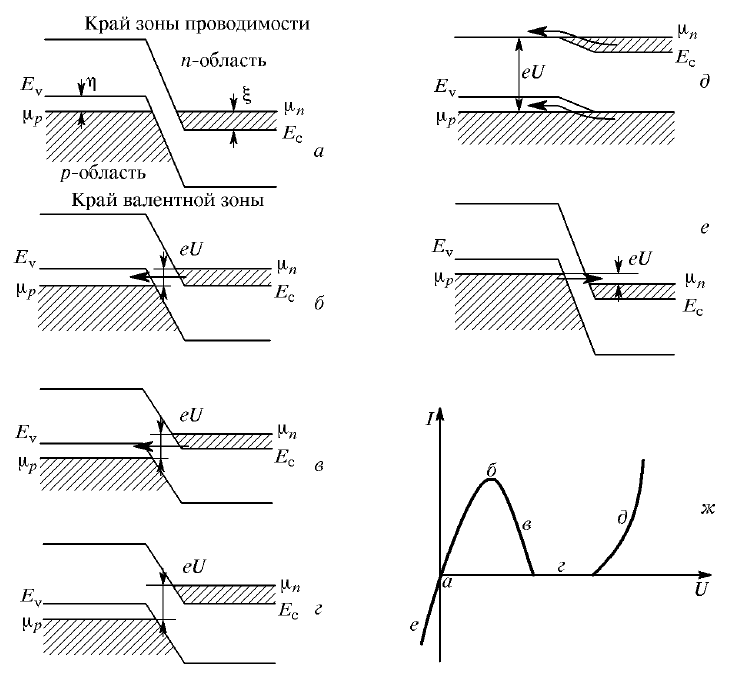
\includegraphics[width=0.5\textwidth]{diode.png}
		\caption{Схема энергетических уровней и вольт-амперная характеристика идеального туннельного диода}
		\label{pic:diode}
	\end{figure}  
	
	Реальная вольт-амперная характеристика туннельного диода отличается от таковой для идеального и представлена на рисунке \ref{pic:not_ideal}. Она учитывает образование примесных зон и возможность их слияния с основными, что объясняет наличия ненулевого тока $I_v$ в минимуме характеристики. 
	
	\begin{figure}[h]
		\centering	
		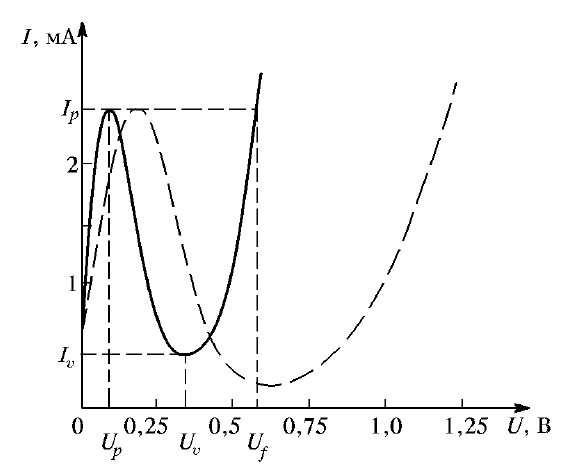
\includegraphics[width=0.4\textwidth]{not_ideal.png}
		\caption{Вольт-амперная характеристика неидеальных туннельных диодов с меньшей (сплошная линия) и большей (пунктирная линия) шириной запрещенной зоны}
		\label{pic:not_ideal}
	\end{figure}  
	
	Вольт-амперная характеристика реального туннельного диода (см. рисунок \ref{pic:not_ideal}) описывается следующими значениями напряжения и тока. 
	
	Напряжению $U_p$ соответствует максимум тока $I_p$, при котором смещение энергетических зон одинаково, причем это напряжение связано с расстоянием $\xi$ между уровнем Ферми в $n$-области и зоной проводимости и энергией $E_\text{n max}$, соответствующей максимуму плотности распределения электронов, следующим отношением: 
	
	\[ U_p \approx \frac{\xi - E_\text{n max}}{e} \]
	
	В точке $U_v$ ток минимален, и, как следует из описания выше:
	
	\[ U_v \approx \frac{(\mu_n - E_c) + (E_v - \mu_p)}{e} = \frac{\xi + \eta}{e} \approx \frac{2\xi}{e} \approx \frac{2\eta}{e} \]
	
	Напряжение $U_f$ характеризует раствор вольт-амперной характеристики и определяется шириной запрещенной зоны. 


\section{Экспериментальная установка}
	
	Схема установки представлена на рисунке \ref{pic:scheme_oscil}. На вход $ Y $ осциллографа подается напряжение, пропорциональное току через диод, а на вход $ X $ --- падение напряжения на диоде.
	
	\begin{figure}[h]
		\centering	
		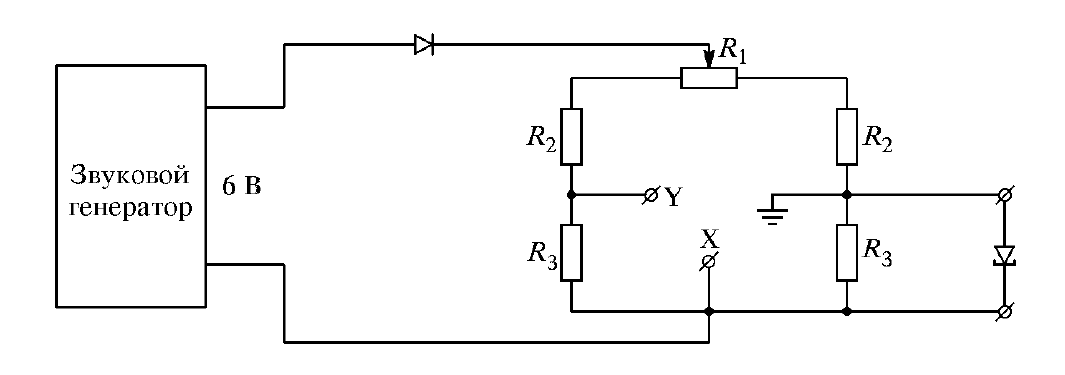
\includegraphics[width=0.5\textwidth]{scheme_oscil.png}
		\caption{Схема наблюдения вольт-амперной характеристики туннельного диода с помощью осциллографа}
		\label{pic:scheme_oscil}
	\end{figure}
	
	Ток $I$ через диод зависит от напряжения $U$ на нем по следующей формуле: 
	
	\[ I = U \frac{R_1 + 2(R_2 + R_3)}{(R_1 + 2R_2) \cdot R_3} \]
	

\section{Ход работы}

Сопротивления нашей установки:
$$R_1 = 680 \text{ Ом}$$
$$R_2 = 100 \text{ Ом}$$
$$R_3 = 120 \text{ Ом}.$$


Изучим вольт-амперную характеристику обыкновенного и туннельного диодов с помощью осциллографа.

\begin{figure}[h!]
    

\begin{minipage}{0.45\textwidth}
  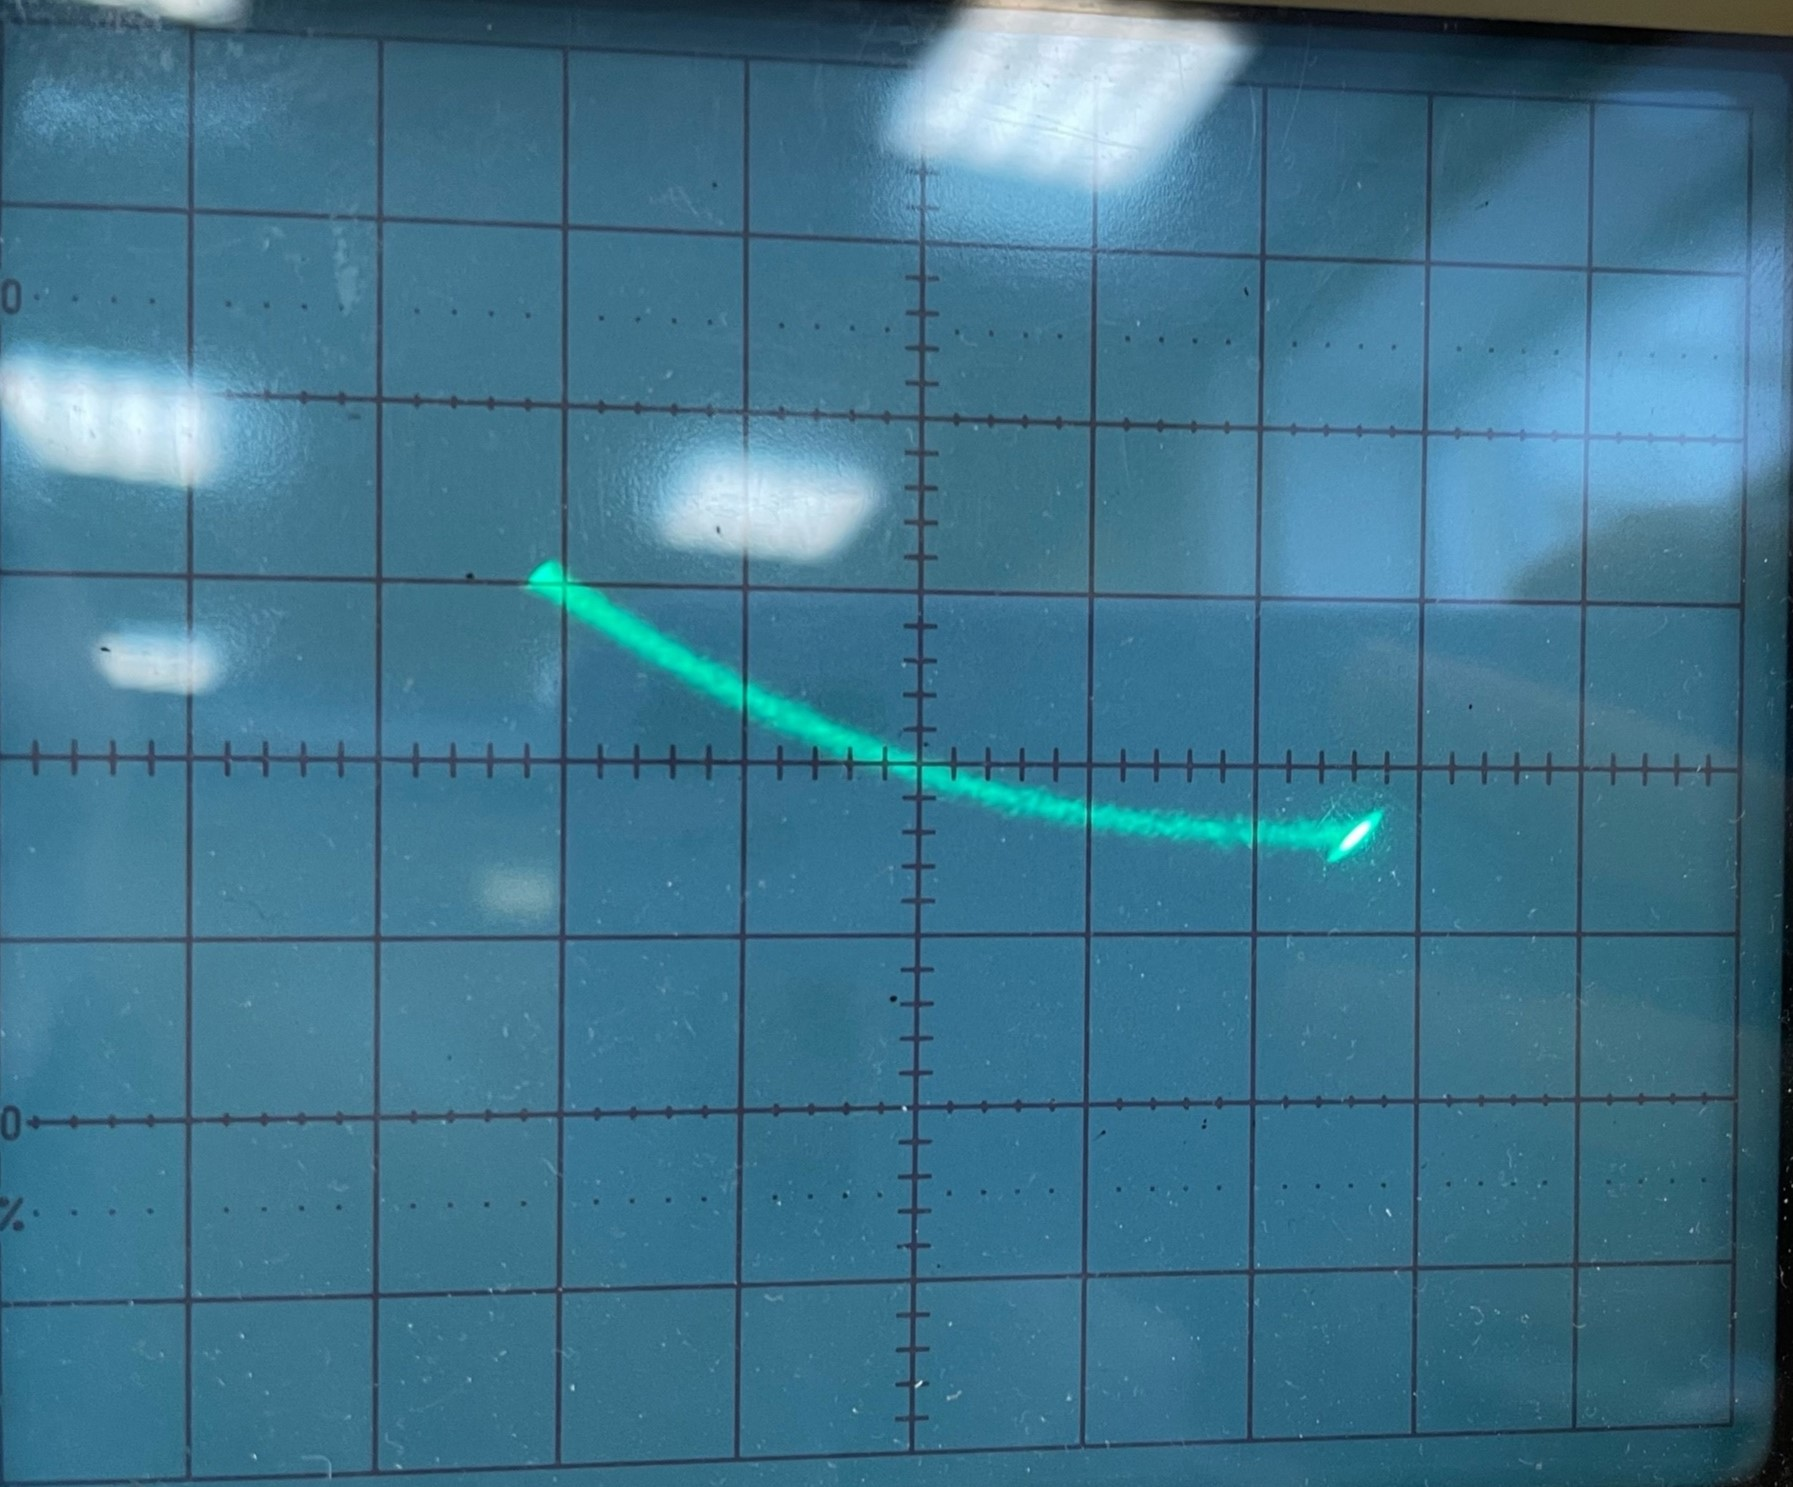
\includegraphics[width= \linewidth]{ваха_обычный.jpg}
  \caption{Вольт-амперная характеристика обычного полупроводникового диода}
  \label{fig:mirrored_polarization_degree_by_theta}

\end{minipage}
\hfill%
\begin{minipage}{0.45\textwidth}
 
  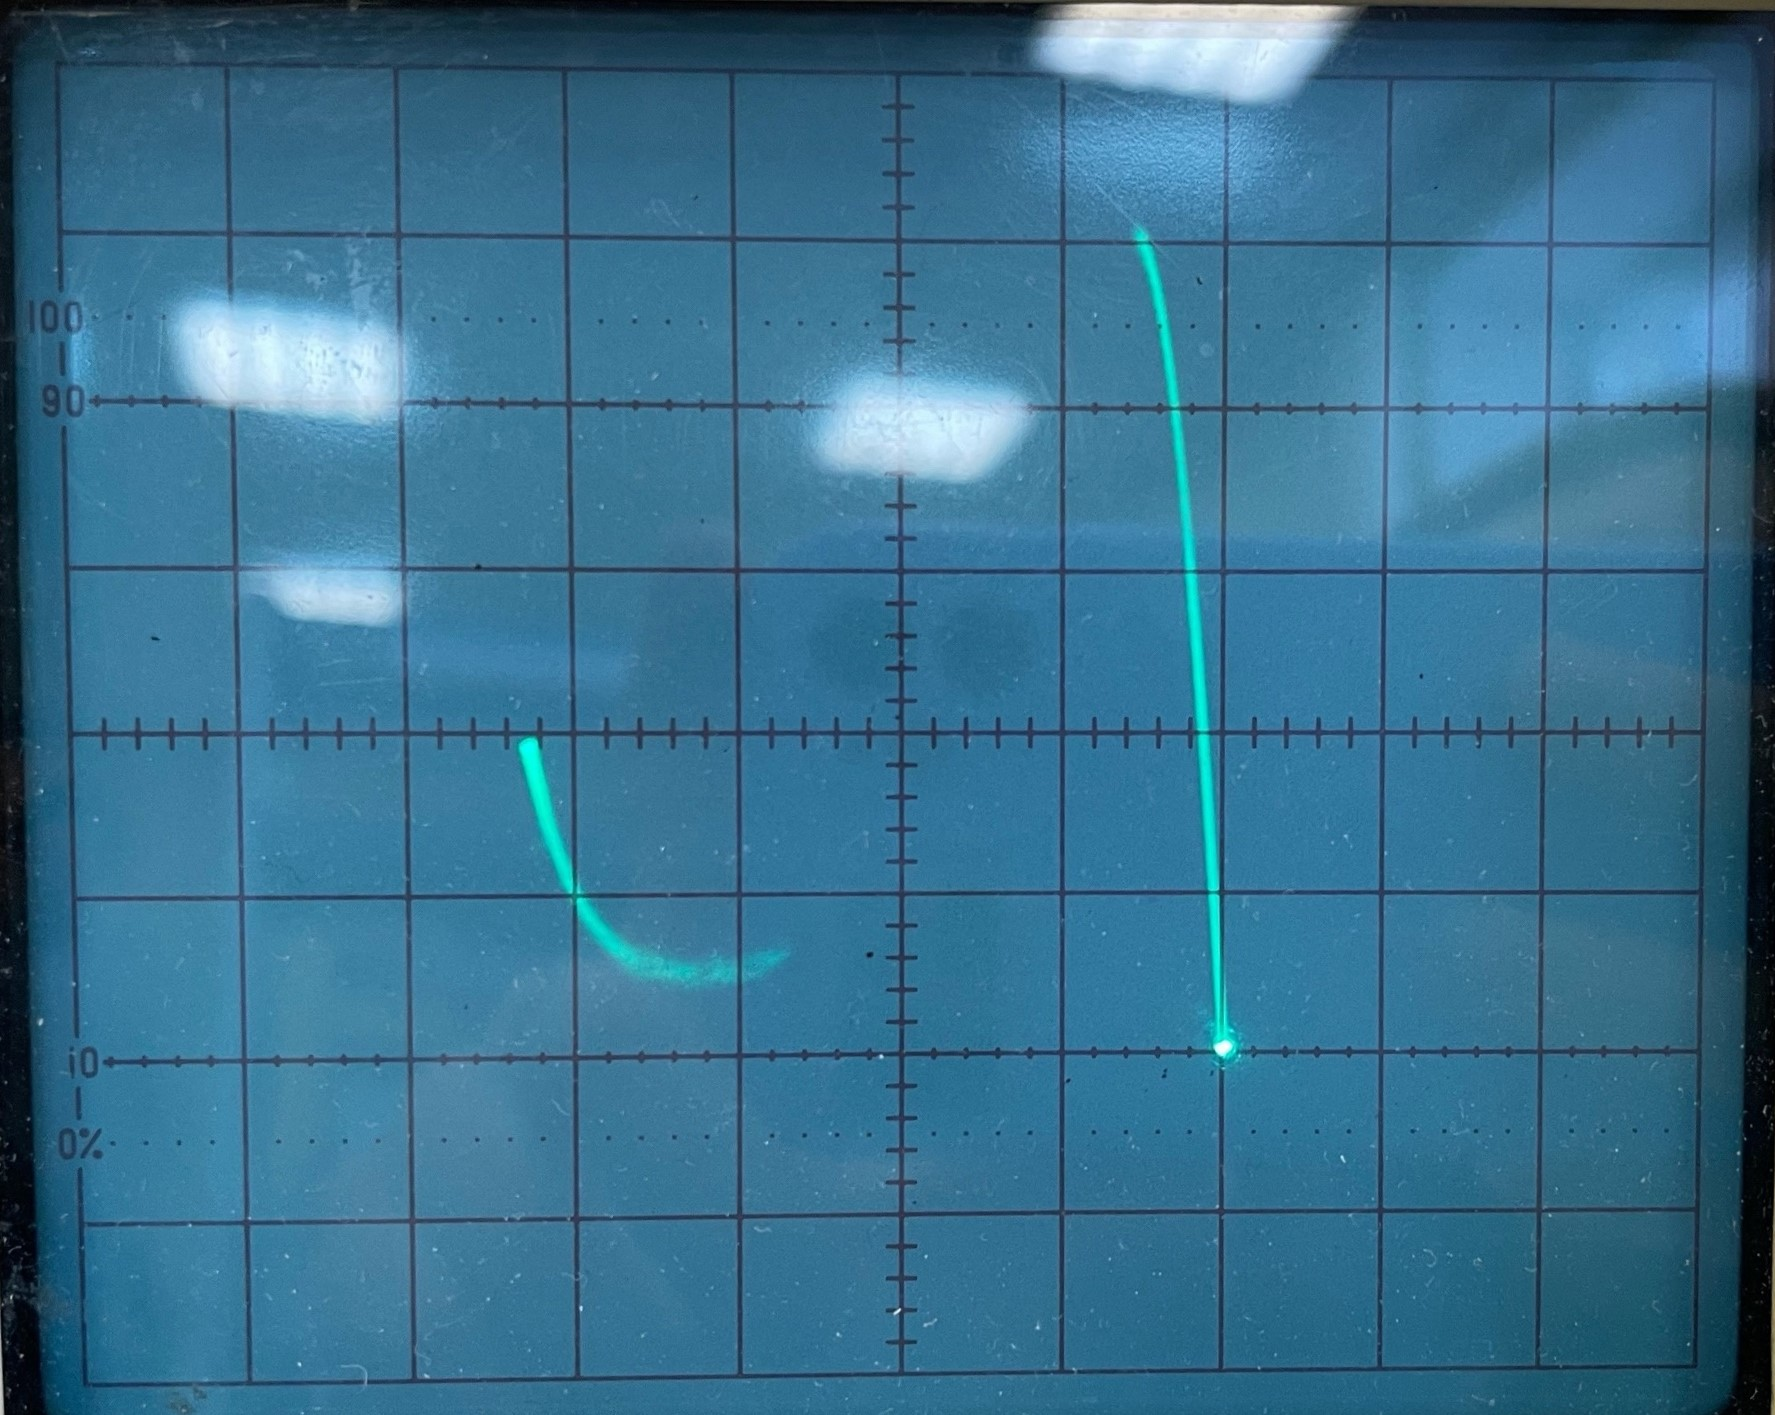
\includegraphics[width= \linewidth]{ваха_туннельный.jpg}
  \caption{Вольт-амперная характеристика туннельного полупроводникового диода}
  \label{fig:duffuse_polarization_degree_by_theta}

\end{minipage}
\end{figure}
Изучим вольт-амперную характеристику обыкновенного и туннельного диодов в статическом режиме.

\begin{figure}[h!]
    

\begin{minipage}{0.5\textwidth}
  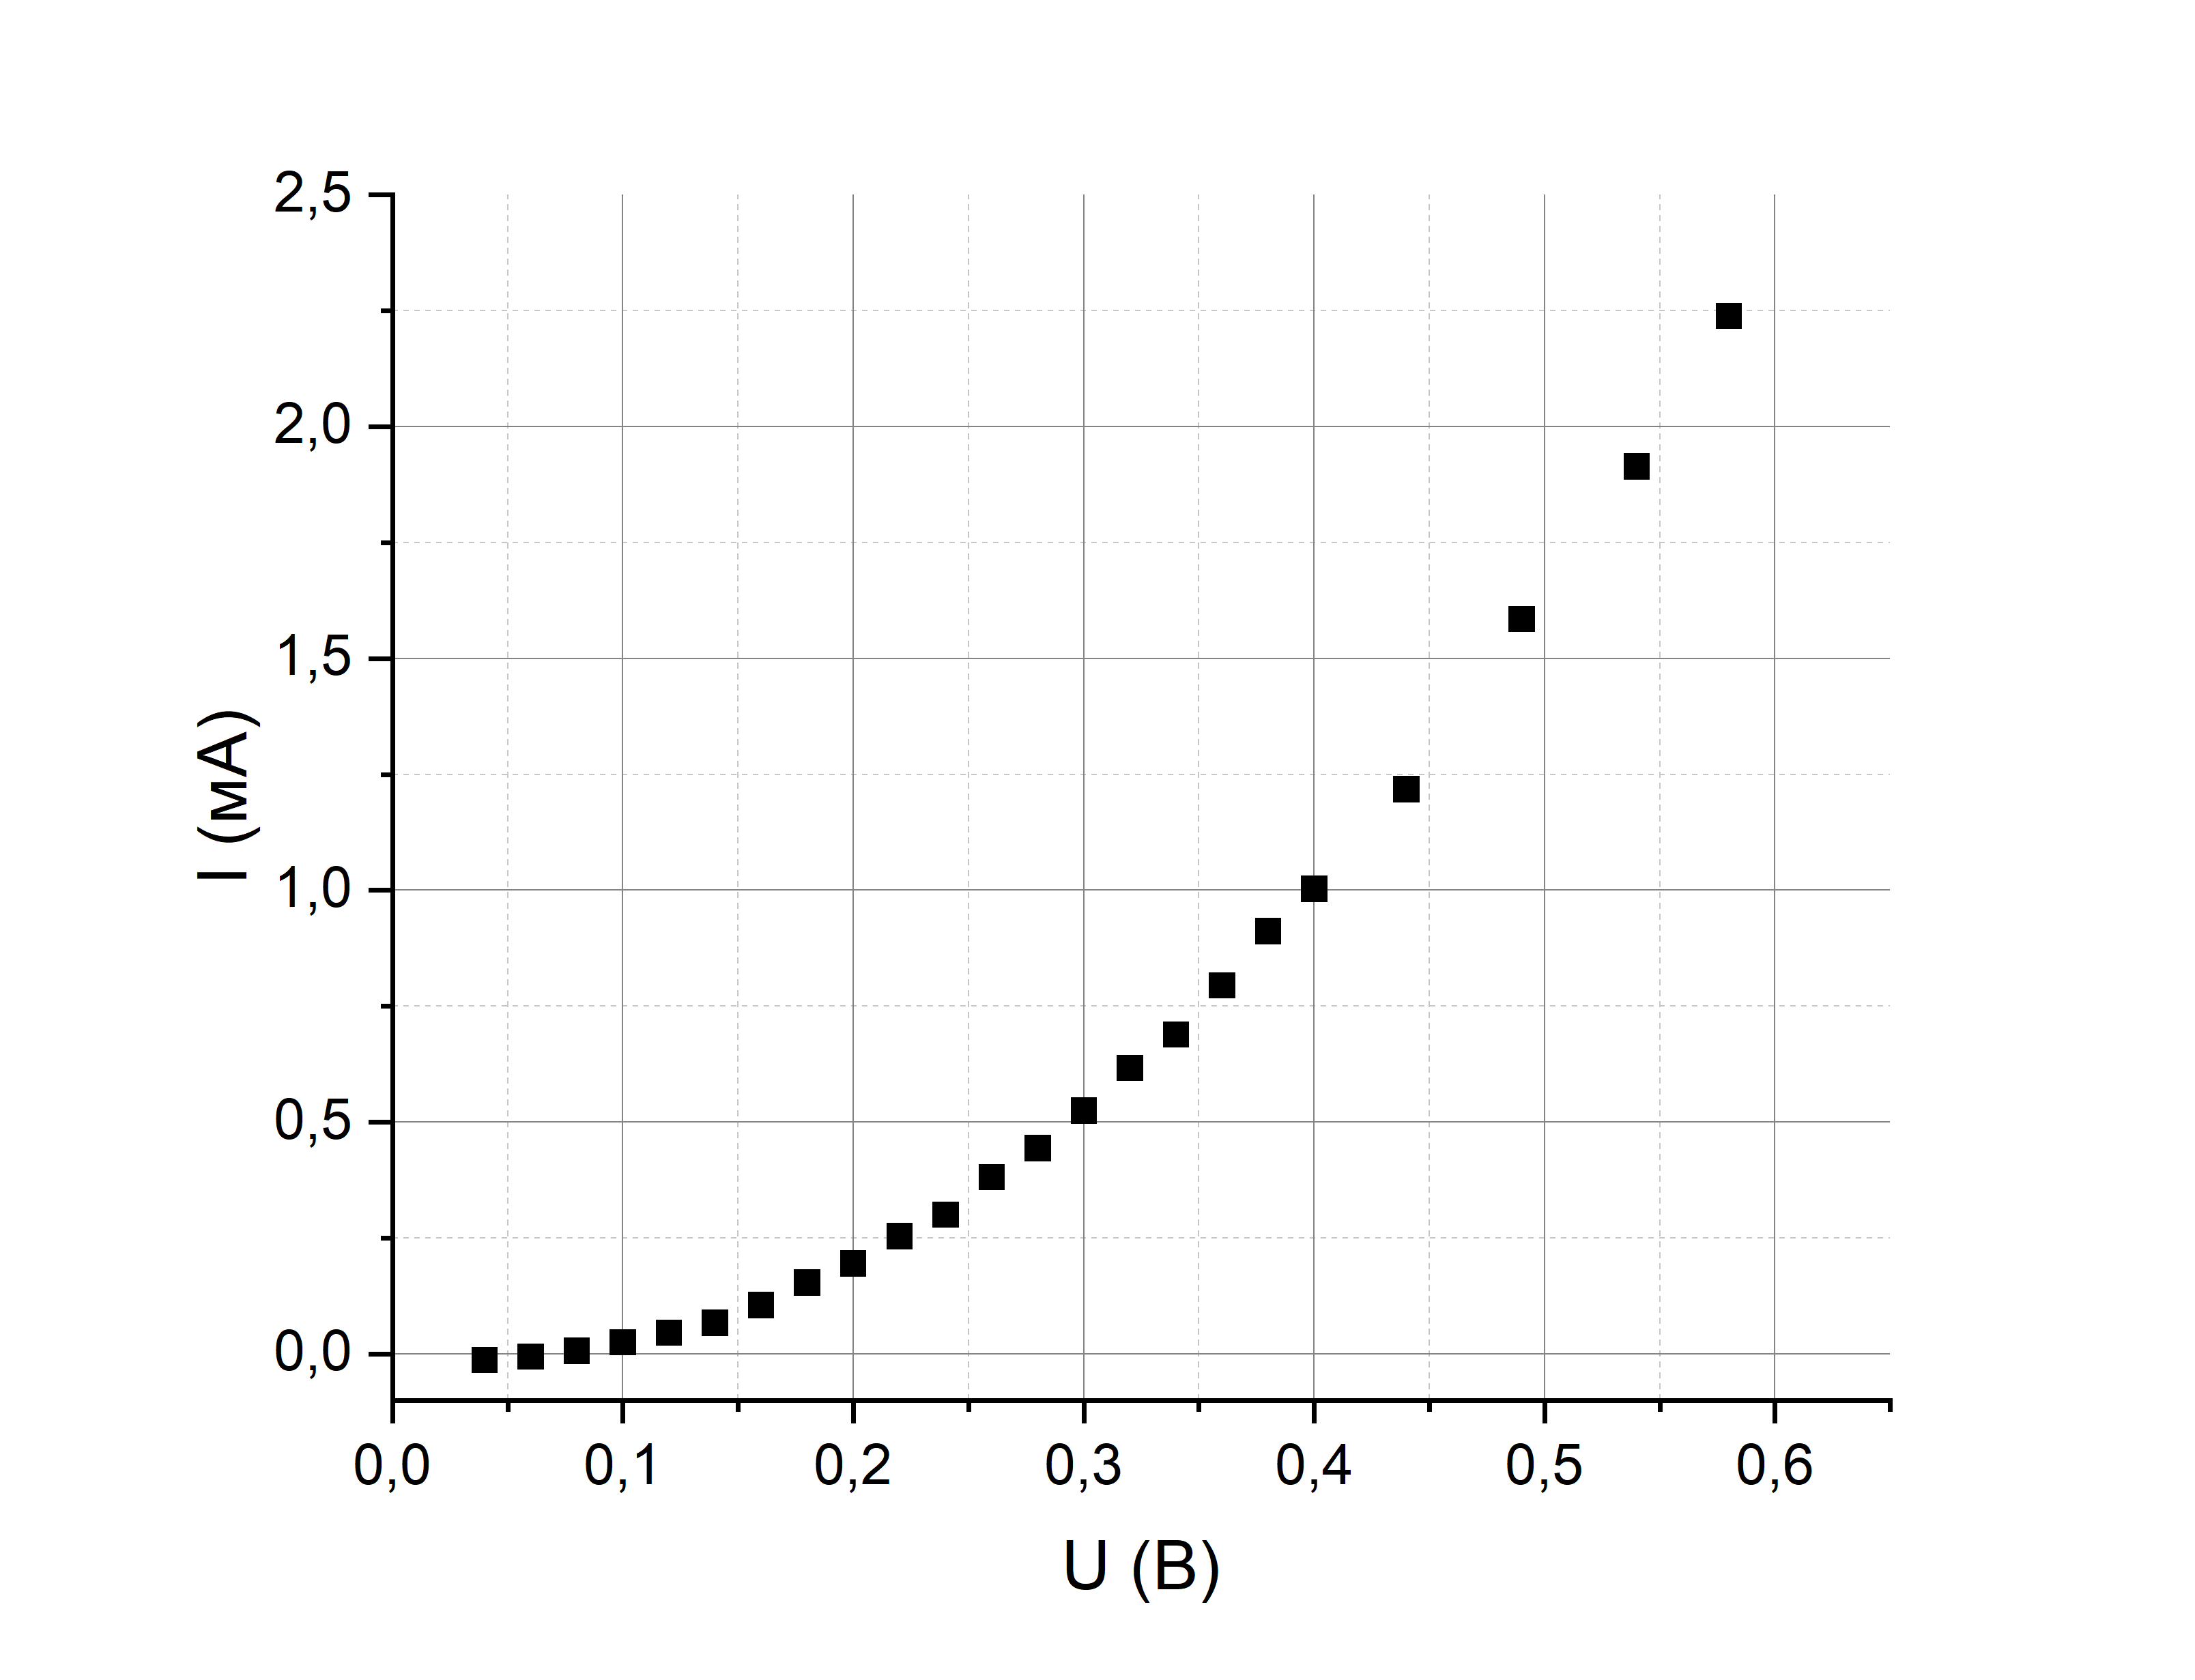
\includegraphics[width= \linewidth]{ordinary.png}
  \caption{Вольт-амперная характеристика обычного полупроводникового диода}
  \label{fig:mirrored_polarization_degree_by_theta}

\end{minipage}
\hfill%
\begin{minipage}{0.5\textwidth}
 
  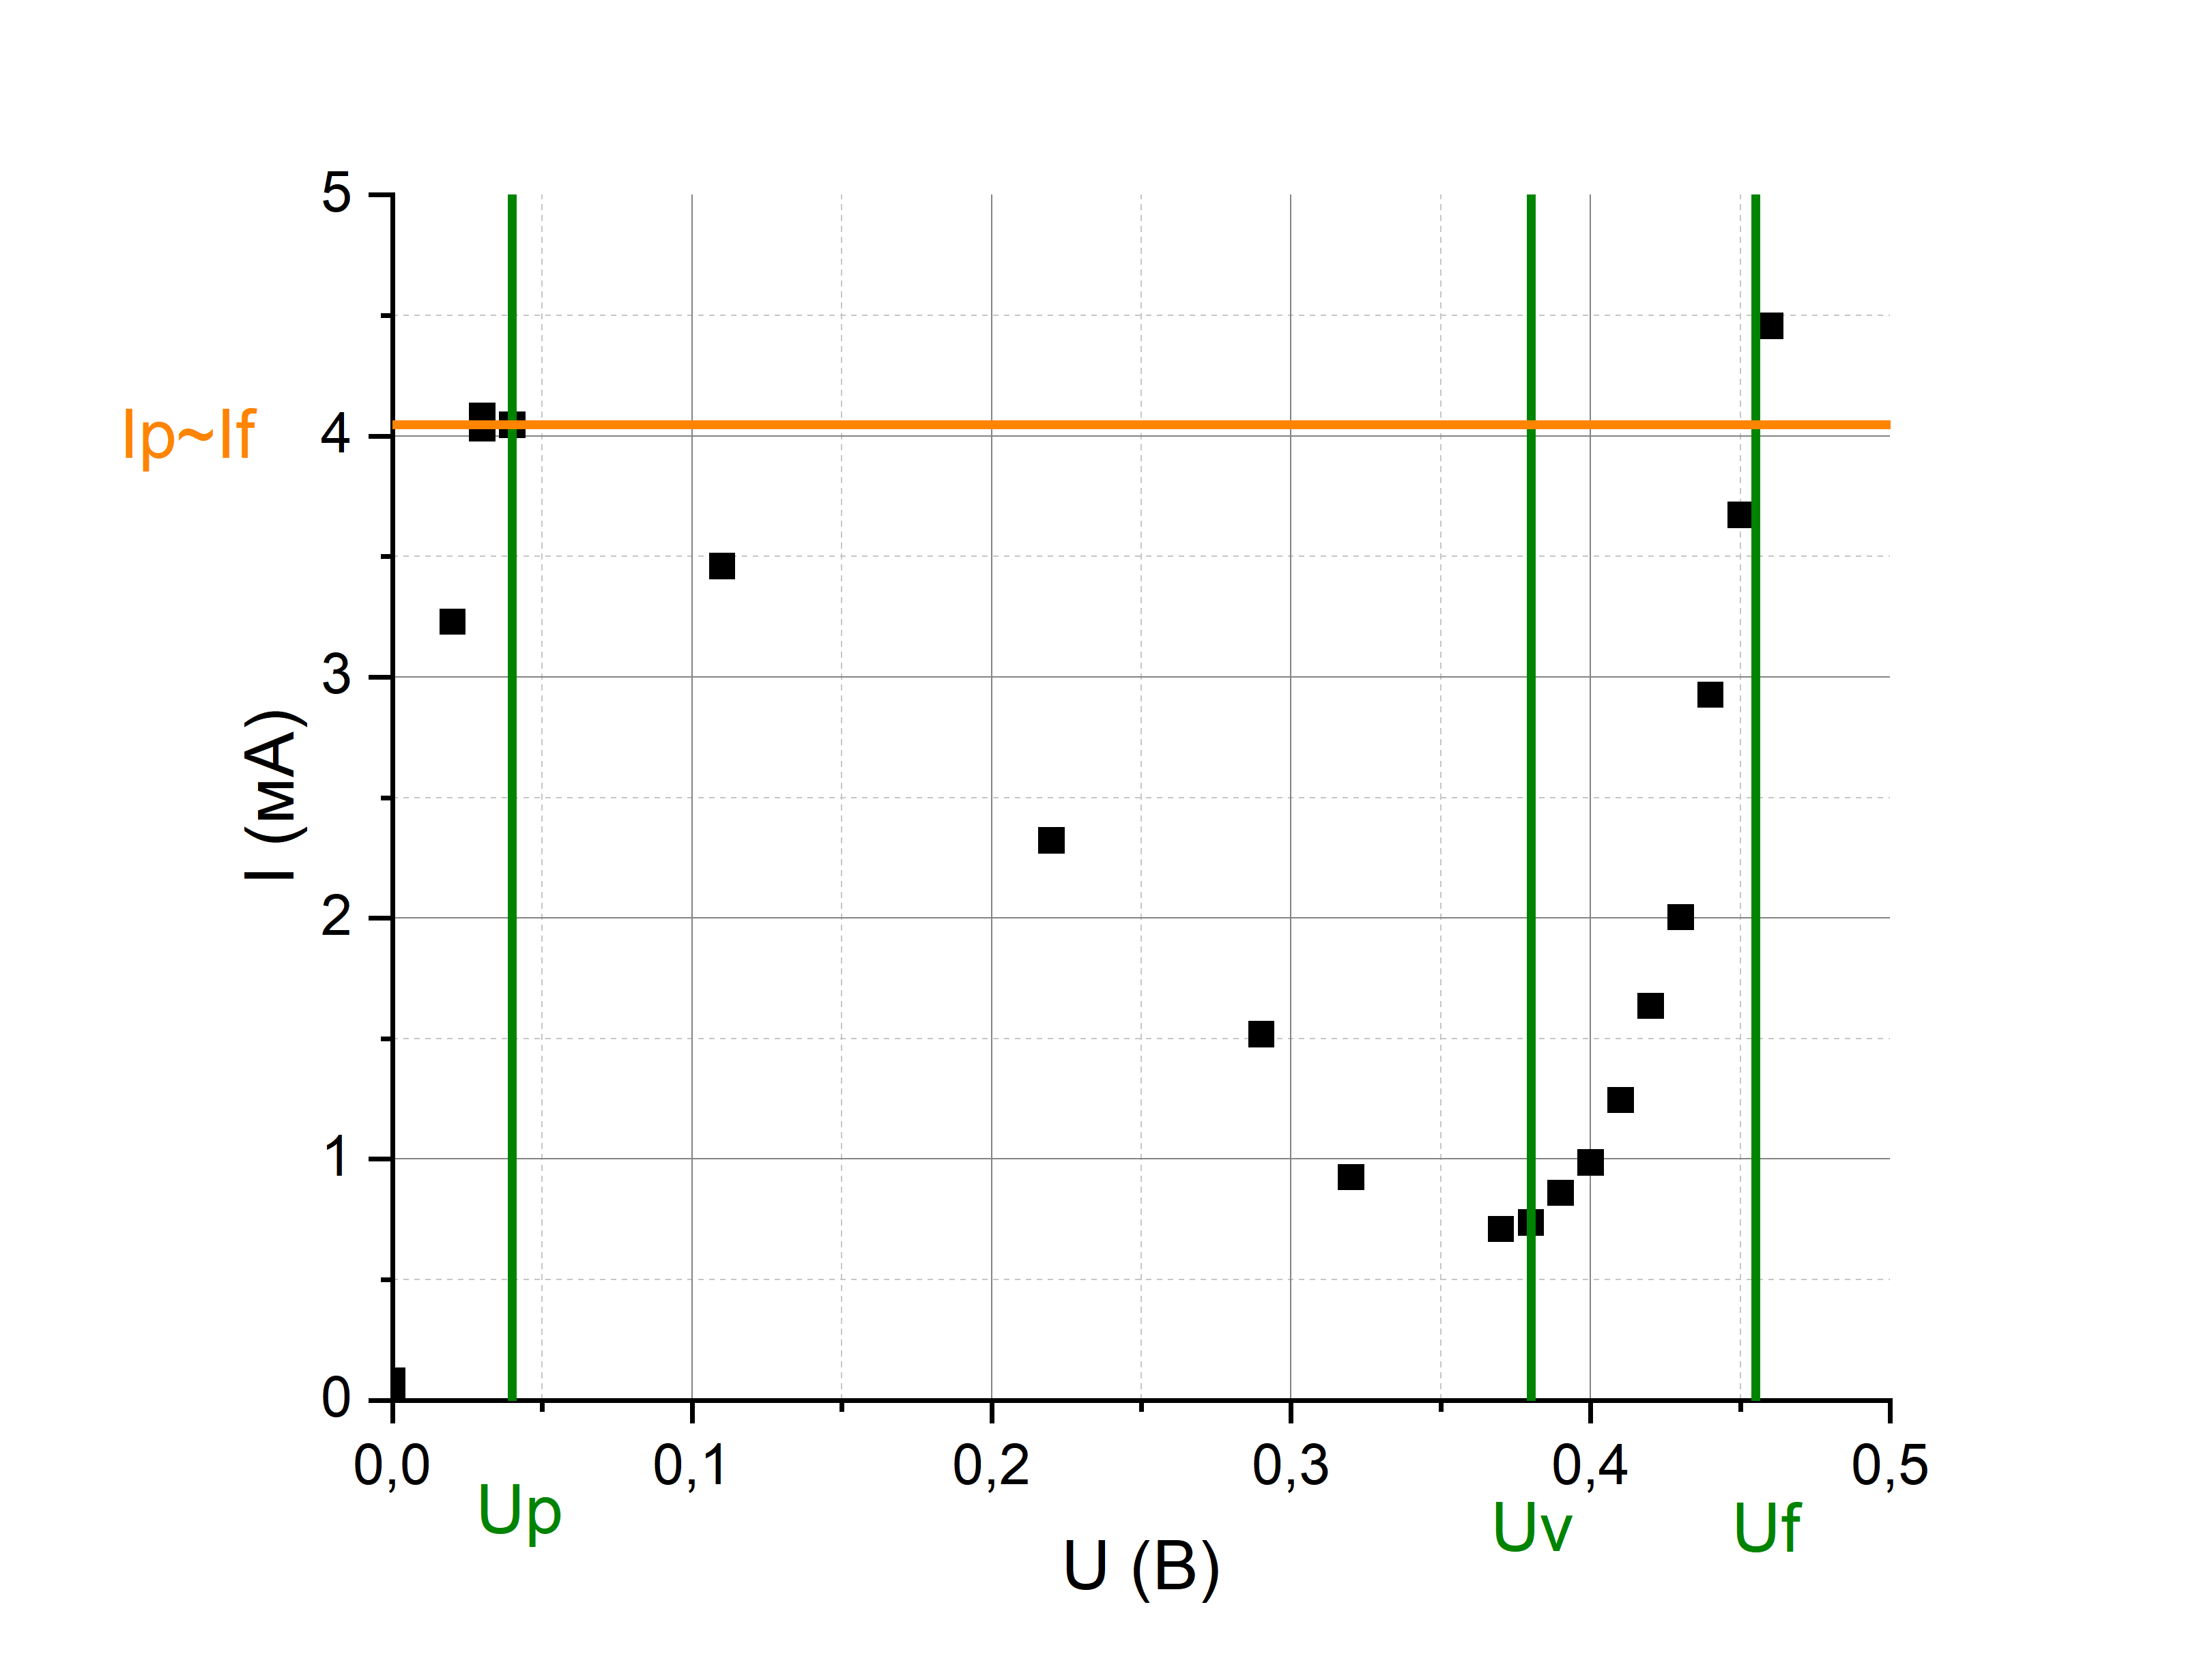
\includegraphics[width= \linewidth]{tunnel.png}
  \caption{Вольт-амперная характеристика туннельного полупроводникового диода}
  \label{fig:duffuse_polarization_degree_by_theta}

\end{minipage}
\end{figure}


Оценим $U_p, U_v$ и $U_f$ из динамической и статической ВАХ.

\begin{table}[h!]
\begin{tabular}{|l|l|l|l|l|l|l|l|l|}
\hline
             & $U_p$, В & $U_v$, В & $U_f$, В & $\sigma_U, $ В & $I_p$, мА & $I_v$, мА & $I_f$, мА & $\sigma_I, $ мА \\ \hline
Динамический & 0,060    & 0,330    &          & 0,020          & 6,400     & 3,500     &           & 0,200           \\ \hline
Статический  & 0,040    & 0,370    & 0,455    & 0,001          & 4,046     & 0,711     & 4,065     & 0,004           \\ \hline
\end{tabular}
\caption{Результаты для $U_p, U_v$ и $U_f$ и $I_p, I_v$ и $I_f$}
\end{table}

Примем $E_v = 0$. Найдем энергию Ферми:
$$\mu_n \approx \mu_p \approx eU_v/2$$

Найдем энергию, соответствующую максимальной плотности распределения электронов $E_{n_{max}}$:

$$E_{n_{max}} = \mu_n - eU_p$$


\begin{table}[h!]
\begin{tabular}{|l|l|}
\hline
Динамический                 & Статический                  \\ \hline
$\mu_n \approx 180$ мэВ     & $\mu_n \approx 185$ мэВ     \\ \hline
$E_{n_{max}} \approx 120$ мэВ & $E_{n_{max}} \approx 145$ мэВ \\ \hline
\end{tabular}
\caption{Характеристики туннельного диода}
\end{table}

\section{Вывод}
В данной работе исследовались ВАХ обыкновенного и туннельного диодов в динамическом и статическом режимах. В отличие от обыкновенного диода, у туннельного наблюдается промежуток спада тока. Также были получены характеристики туннельного диода, они приведены в таблице (2). Полученные в разных режимах результаты схожи между собой, но мы не располагаем данными о диоде, поэтому сравнить их с табличными нет возможности.


\end{document}